\section{Abstract\-Iterator Class Reference}
\label{classAbstractIterator}\index{AbstractIterator@{AbstractIterator}}
{\tt \#include $<$abstractiterator.hpp$>$}

Inheritance diagram for Abstract\-Iterator::\begin{figure}[H]
\begin{center}
\leavevmode
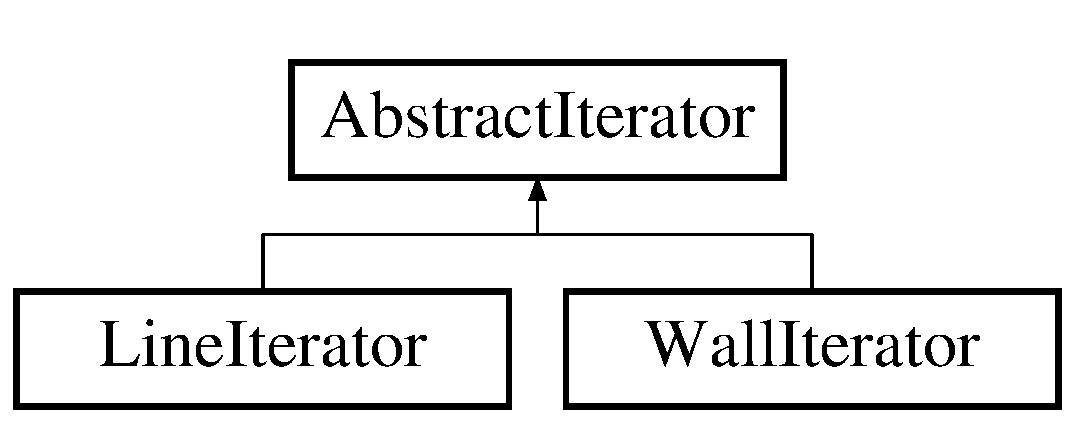
\includegraphics[height=2cm]{classAbstractIterator}
\end{center}
\end{figure}
\subsection*{Public Member Functions}
\begin{CompactItemize}
\item 
virtual bool {\bf operator!} ()=0
\item 
virtual void {\bf operator++} (int)=0
\end{CompactItemize}


\subsection{Detailed Description}
for (Abstract\-Iterator i; !i; i++);



\subsection{Member Function Documentation}
\index{AbstractIterator@{Abstract\-Iterator}!operator"!@{operator"!}}
\index{operator"!@{operator"!}!AbstractIterator@{Abstract\-Iterator}}
\subsubsection{\setlength{\rightskip}{0pt plus 5cm}virtual bool operator! ()\hspace{0.3cm}{\tt  [pure virtual]}}\label{classAbstractIterator_a0}




Implemented in {\bf Line\-Iterator} {\rm (p.\,\pageref{classLineIterator_a1})}, and {\bf Wall\-Iterator} {\rm (p.\,\pageref{classWallIterator_a1})}.\index{AbstractIterator@{Abstract\-Iterator}!operator++@{operator++}}
\index{operator++@{operator++}!AbstractIterator@{Abstract\-Iterator}}
\subsubsection{\setlength{\rightskip}{0pt plus 5cm}virtual void operator++ (int)\hspace{0.3cm}{\tt  [pure virtual]}}\label{classAbstractIterator_a1}




Implemented in {\bf Line\-Iterator} {\rm (p.\,\pageref{classLineIterator_a2})}, and {\bf Wall\-Iterator} {\rm (p.\,\pageref{classWallIterator_a2})}.

The documentation for this class was generated from the following file:\begin{CompactItemize}
\item 
{\bf abstractiterator.hpp}\end{CompactItemize}
